\subsection{Ladeablauf}\label{sec:ladeablauf}

...........Die Betriebszeit des Dojos ermöglicht eine Betriebszeit von fünf Stunden, wobei durch Ladezyklen zwischen den Besuchen eine ganztägiger Betrieb ermöglicht wird. Darum wurde im Ziel 5.1 ein Arbeitstag genannt. Um dies zu veranschaulichen, gibt nachfolgende Abbildung \ref{fig:Ladezyklus Dojo} einen Einblick ins Konzept.

\begin{figure}[H]
	\begin{center}
		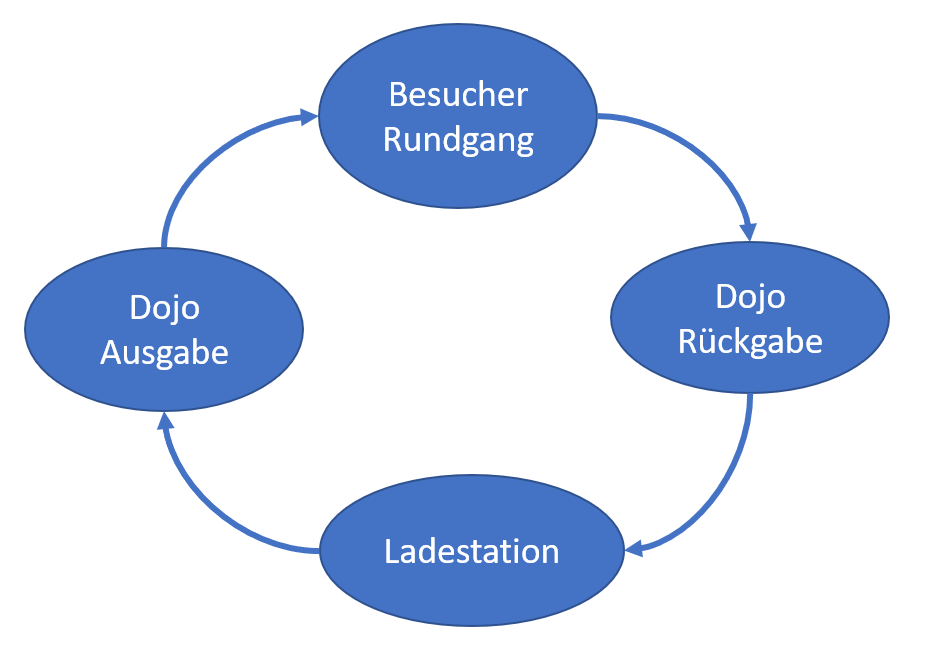
\includegraphics[width=120mm]{data/LadezyklusDojo.png}
		\caption[Ladezyklus Dojo]{Ladezyklus Dojo} %picture caption
		\label{fig:Ladezyklus Dojo}
	\end{center}
\end{figure}

Wie bereits oben beschrieben, beträgt die Betriebszeit eines durchschnittlichen Rundganges rund drei bis vier Stunden. Sobald die Rückgabe erfolgt ist, wird das Dojo in die Ladebuchse gesteckt wobei immer diese Dojos rausgegeben werden, welche sich am längsten in der Ladestation befinden. Bei einer Stückzahl welche grösser ist als die Besucherzahl, erlaubt dies einen lückenlosen Betrieb.
\cite{Plank}
\ref{sec:bluetooth}
